% contient une description du fonctionnement de Szeliski, pour préciser qu'on possède une méthode "parfaite" dans le cas des affinités
\subsubsection{Principe général}
	
	Les affinités sont un cas particulier d'homographie. Elles peuvent être traitées par une méthode multi-étape qui ne crée pratiquement aucun \emph{aliasing} \cite{szeliski2010high}.
	
	Le principe de cette méthode est de d'abord se ramener à des affinités qui n'agissent que selon une direction (affinités de la forme $\pmatrice{a_0 & a_1 & t\\ 0 & 1 & 0}$ ou $\pmatrice{1 & 0 & 0\\ a_1 & a_0 & t}$). Par abus de langage, on parlera de \emph{shear}, bien qu'il s'agisse de la composée d'un cisaillement, d'une dilatation unidirectionnelle et d'une translation, tous dans la même direction. Chacun des \emph{shears} est alors effectué en trois étapes : un sur-échantillonnage dans la direction transverse, un \emph{shear} et un sous-échantillonnage dans la direction transverse.
	
	Le principe de la méthode est en fait de choisir le facteur de sur-échantillonnage suffisamment grand pour que l'opération globale se fasse sans \emph{aliasing}, i.e. sans repliement du spectre (figures \ref{szeliski_decompoNaive} et \ref{szeliski_decompoSzeliski}).
		
	\begin{figure}
		\centering
		\subfigure[Spectre de l'image d'entrée]{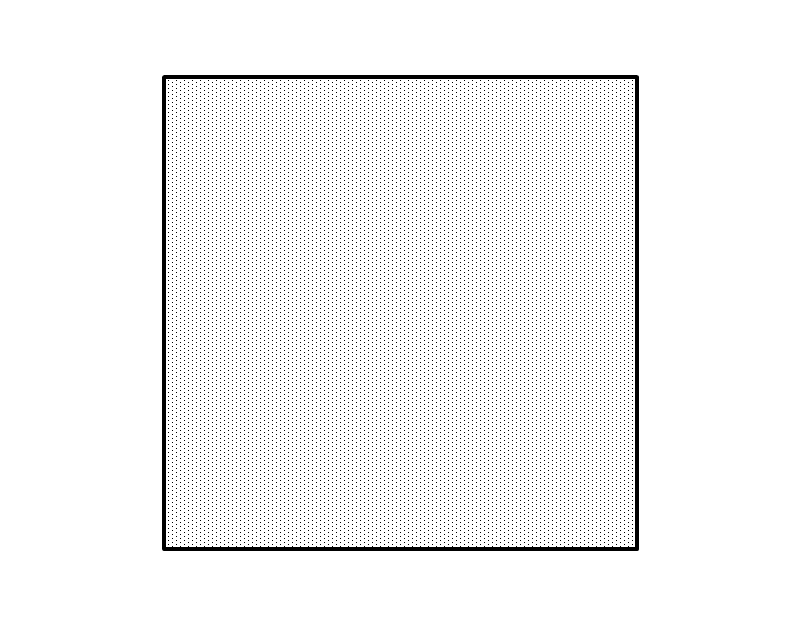
\includegraphics[scale=0.5]{szeliski_naiveEntree.png}}
		\subfigure[Spectre de l'image de sortie : repliement du spectre]{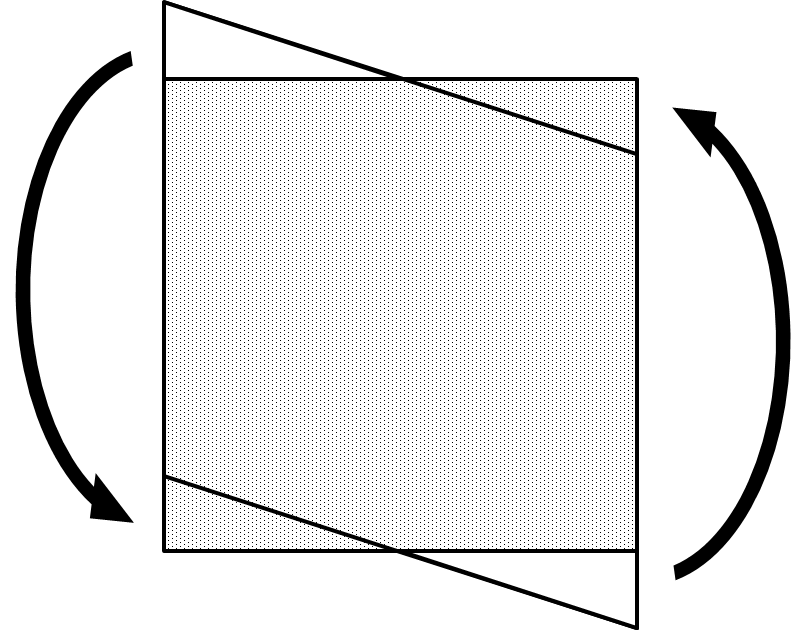
\includegraphics[scale=0.5]{szeliski_naiveSortie.png}}
		\caption{Effet d'un \emph{shear} sur le spectre de l'image (par la méthode naïve)}
		\label{szeliski_decompoNaive}
	\end{figure}
		
	\begin{figure}
		\centering
		\subfigure[Spectre de l'image d'entrée]{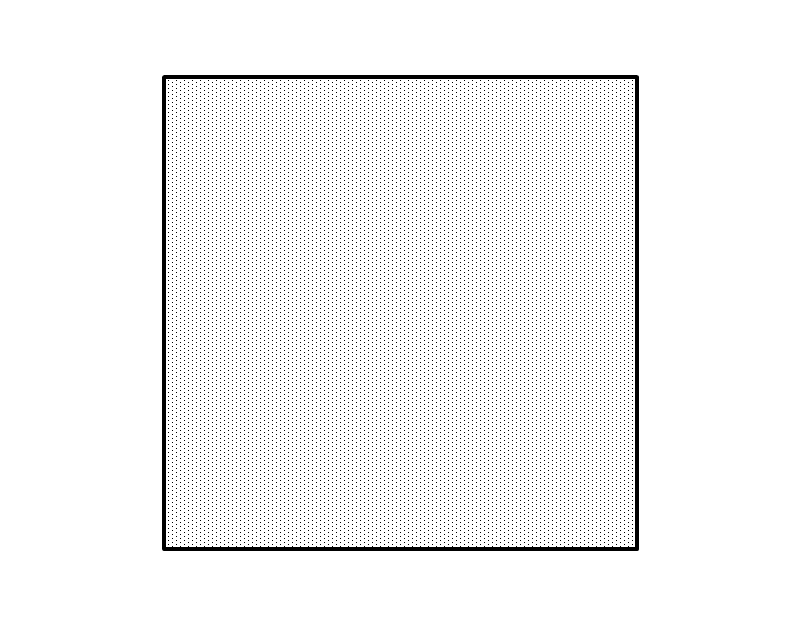
\includegraphics[scale=0.5]{szeliski_szeliskiEntree.png}}
		\subfigure[Spectre de l'image après sur-échantillonnage]{
\includegraphics[scale=0.5]{szeliski_szeliskiSurechantillonnage.png}}
		\subfigure[Spectre de l'image après sur-échantillonnage et \emph{shear}]{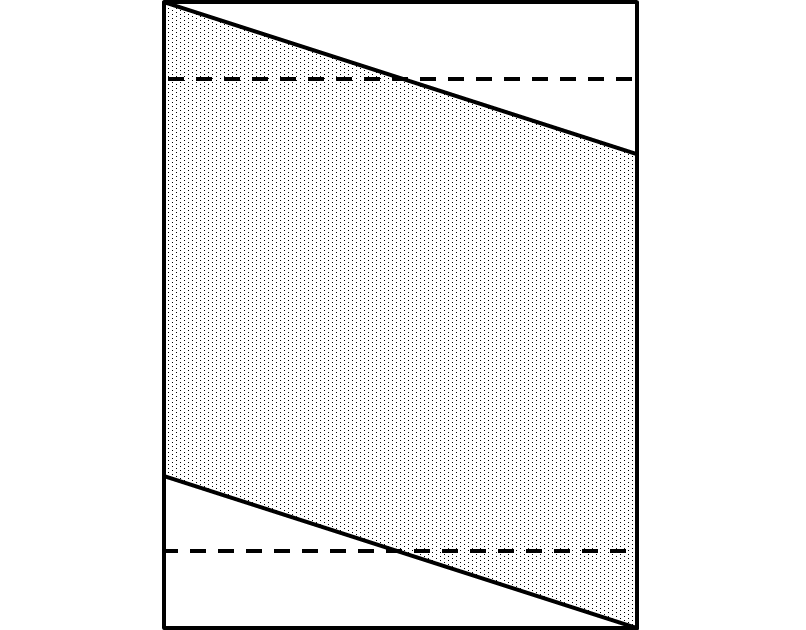
\includegraphics[scale=0.5]{szeliski_szeliskiShear.png}}
		\subfigure[Spectre de l'image de sortie (après sur-échantillonnage, \emph{shear} et sous-échantillonnage)]{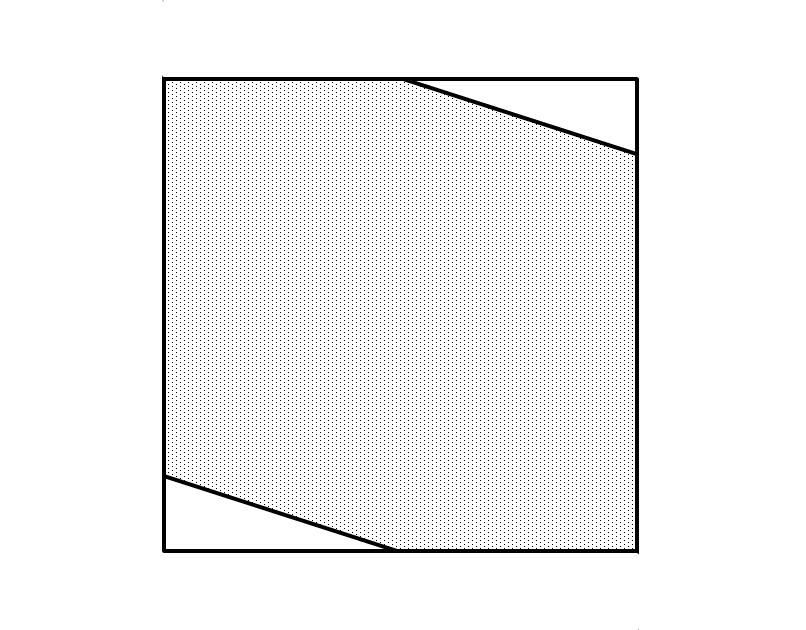
\includegraphics[scale=0.5]{szeliski_szeliskiSortie.png}}
		\caption{Effet d'un \emph{shear} sur le spectre de l'image (par la décomposition en plusieurs étapes)}
		\label{szeliski_decompoSzeliski}
	\end{figure}
	
	Ces trois opérations sont toutes des \emph{shears} (éventuellement réduit à une dilatation) et seront nommées $\mathcal R$ ; selon qu'elles modifient l'image verticalement (en laissant l'abscisse inchangée) ou horizontalement (en laissant l'ordonnée inchangée), on parlera de $\mathcal R_v$ ou de $\mathcal R_h$ . Ces opérations $\mathcal R$ sont réalisées par une convolution par un noyau d'interpolation, en l'occurrence une fonction de type \emph{raised cosine}.
	\[h : x \mapsto \sinc(\frac{x}{T})\frac{\cos(\frac{\pi\beta x}{T})}{1-\frac{4\beta^2x^2}{T^2}}\]
	On modifie éventuellement, selon les coefficients du \emph{shear}, la taille du support du filtre (en appelant $h(\frac{x}{s})$ au lieu de $h(x)$, avec $s\geq 1$). Cela permet, en cas de sur-échantillonnage, d'avoir une protection contre l'\emph{aliasing}. Le coefficient $s$ dépend aussi des \emph{fréquences conservées maximales} $u_{max}$ et $v_{max}$ qui seront définies et expliquées plus loin.
	
	On est ainsi capable d'effectuer, en trois étapes $\mathcal R$ et sans \emph{aliasing}, tous les \emph{shears}. Or une affinité se décompose toujours en deux \emph{shears}, on peut donc toujours traiter une affinité quelconque, et ce, sans \emph{aliasing}.
	
	Cette méthode semble donc décomposer une affinité en 6 opérations $\mathcal R$ (3 pour chacun des 2 \emph{shears}) ; en pratique, il est possible de réunir certains $\mathcal R$, s'ils sont dans la même direction. La décomposition peut alors se réduire à 4 opérations $\mathcal R$ : un sur-échantillonnage vertical, un \emph{shear} horizontal, un \emph{shear} vertical puis enfin un sous-échantillonnage horizontal.
	
\subsubsection{Étapes de l'algorithme}
	On détaille donc ici les étapes de l'algorithme de traitement d'une affinité par cette méthode multi-étape. Le pseudo-code correspondant est présent en annexe (algorithmes \ref{szeliski_rh}, \ref{szeliski_rv} et \ref{szeliski_affine}).
	
	On suppose avoir reçu en entrée une image à modifier et la matrice $A$ correspondant à l'affinité inverse que celle à effectuer : l'antécédent du point $(i,j)$ de l'image de sortie se situe donc en $A(i,j)$ sur l'image d'entrée.
	
	On notera
	\[A = \pmatrice{a_{00} & a_{01} & t_0\\ a_{10} & a_{11} & t_1}\]
	
	\paragraph{Éventuelle transposition}
		
		Les $\mathcal R$ peuvent, si l'affinité est par exemple une rotation d'angle $\frac{\pi}{2}$, compresser l'image sur peut de pixels puis tenter de la dilater ; cet effet est un \emph{bottleneck problem} (faut-il le traduire \red{problème d'embouteillage} ?) déjà connu \cite{wolberg1990digital}.
		
		On effectue donc éventuellement une transposition (de l'image et de la matrice) pour éviter cet effet : en notant
		\[\hat a_{00} = \frac{a_{00}}{\sqrt{a_{00}^2+a_{11}^2}}\]
		\[\hat a_{01} = \frac{a_{01}}{\sqrt{a_{00}^2+a_{11}^2}}\]
		\[\hat a_{10} = \frac{a_{10}}{\sqrt{a_{10}^2+a_{11}^2}}\]
		\[\hat a_{11} = \frac{a_{11}}{\sqrt{a_{10}^2+a_{11}^2}}\]
		on transpose dans le cas où $|\hat a_{00}|+|\hat a_{11}|<|\hat a_{01}|+|\hat a_{10}|$.
		
	\paragraph{Décomposition de $A$}
		
		On introduit les fréquences conservées maximales $u_{max}$, $v_{max}$ : ce sont les fréquences, horizontales et verticales, au delà desquelles les fréquences seront effacées par l'application de $A$ ; elles sont donc définies dans le domaine de Fourier par la figure \ref{uMax_vMax}. Les fréquences au delà de $u_{max}$ horizontalement et de $v_{max}$ verticalement peuvent donc être filtrées, cela ne changera pas le spectre de sortie. Ces définitions se font après après avoir ramené le spectre sur le carré $[-1,1]^2$.
		
		\begin{figure}
		\centering
		\subfigure[Spectre de l'image d'entrée]{
\includegraphics[scale=0.5]{uMax_vMax_spectreEntree.png}}
		\subfigure[Spectre de l'image de sortie]{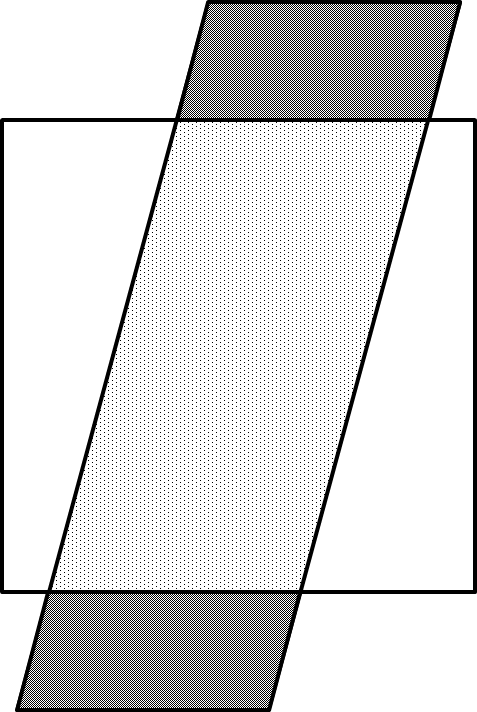
\includegraphics[scale=0.5]{uMax_vMax_spectreSortie.png}}
		\subfigure[Spectre de l'image d'entrée]{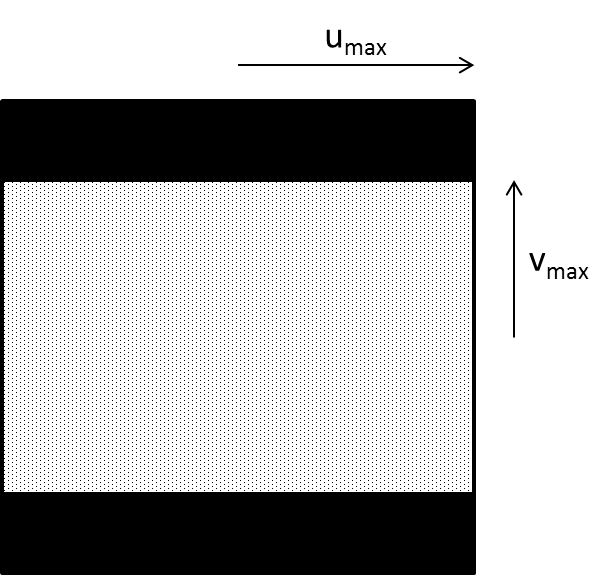
\includegraphics[scale=0.5]{uMax_vMax_spectreUtile.png}}
		\caption{Fréquences conservées par l'affinité. Les zones noires sont les fréquences qui ne seront pas conservées par l'application de l'affinité}
		\label{uMax_vMax}
		\end{figure}
		
		En pratique, $u_{max}$ et $v_{max}$ s'obtiennent en intersectant le spectre d'entrée (le carré $[-1,1]^2$) et l'image réciproque du carré $[-1,1]^2$ par $^t\!A$ (qui correspond à l'opération dans Fourier ; comme précédemment $A$ désigne l'inverse de l'affinité qu'on applique à l'image).
		
		À partir des coefficients de $A$ et des valeurs de $u_{max}$ et $v_{max}$, on peut en déduire les coefficients de sur-échantillonnage verticaux et horizontaux nécessaires \cite{szeliski2010high} :
		\[r_v \geq \max (1,|a_{01}|u_{max}+\min (1,|a_{11}|v_{max}))\]
		\[r_h \geq \max (1,|a_{10}/a_{11}|r_vv_{max}+\min (1,|b_0|u_{max}))\]
		Pour des raisons géométriques, on peut toujours réduire les sur-échantillonnages à $r_h \leq 3$ et $r_v \leq 3$. En effet, pour chacune des deux opérations unidirectionnelles (celles qui seront décomposées en trois $\mathcal R$), le $r_h$ (respectivement $r_v$) peut être réduit à 3, grâce au filtrage qui atténue les fréquences au delà de $u_{max}$ (respectivement $v_{max}$). La figure \ref{rvleq3} présente ce raisonnement géométrique pour une opération sur les colonnes (qui se traduit par une opération sur les lignes dans le domaine de Fourier).
		
		\begin{figure}
		\centering
		\subfigure[$r_v$ non majoré]{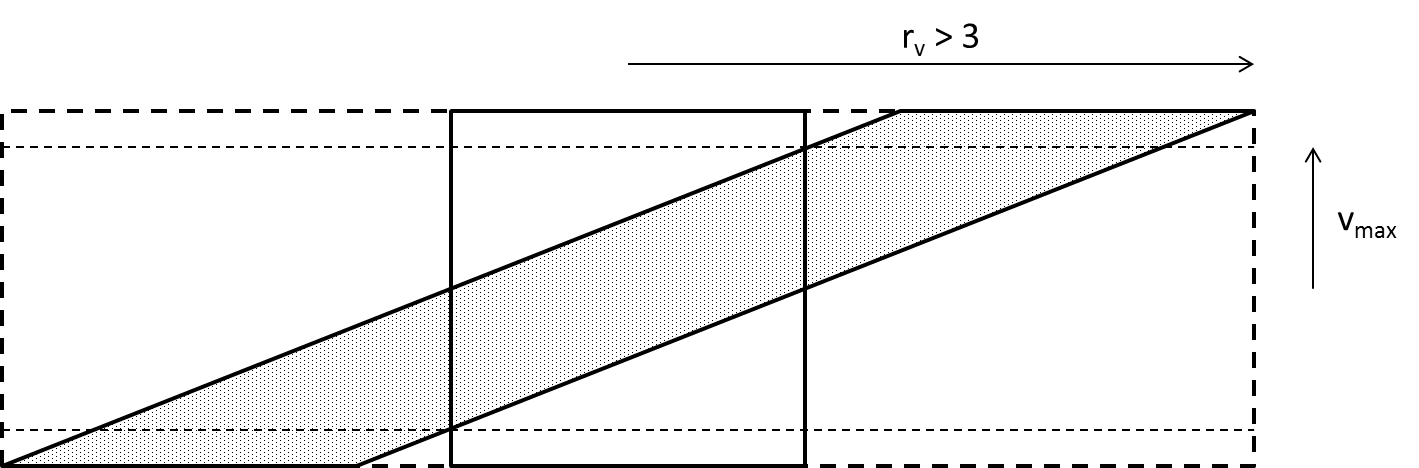
\includegraphics[width=120mm]{rvleq3_notrvleq3.png}}
		\subfigure[$r_v$ majoré par 3 ; on utilise le fait que les distances horizontales sont inchangées]{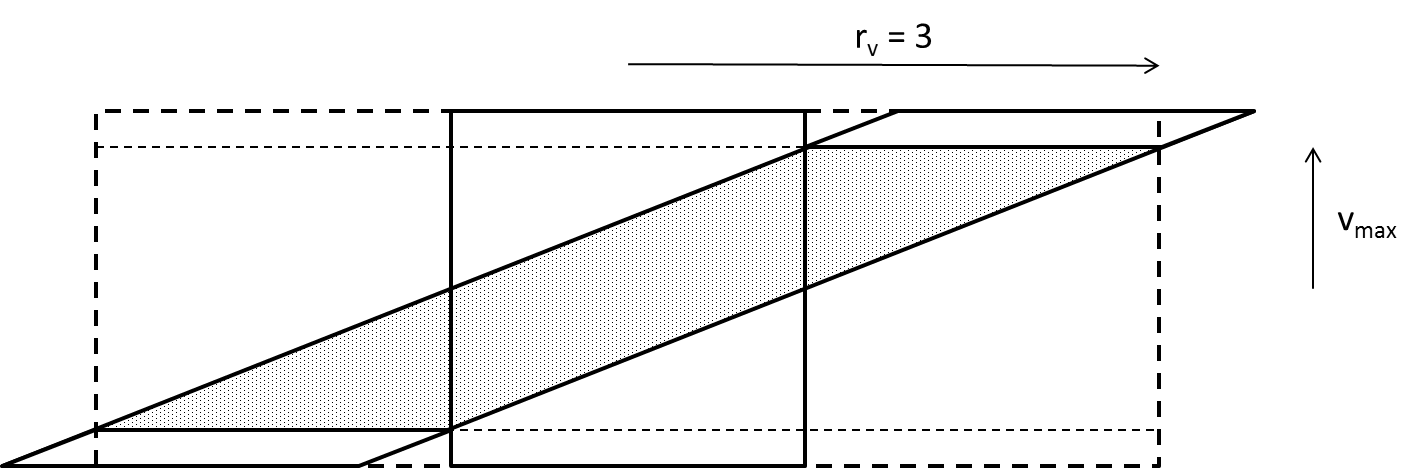
\includegraphics[width=120mm]{rvleq3_rveq3.png}}
		\caption{Réduction de $r_v$ jusqu'à $r_v \leq 3$. Au-delà de $v_{max}$, le filtre efface (atténue) les fréquences, permettant la réduction de $r_v$. $r_v$ est le quotient de la longueur du rectangle pointillé (spectre après suréchantillonnage) par celle du carré (spectre initial)}
		\label{rvleq3}
		\end{figure}
		
		On décompose alors $A$ en :
		\[
			A = \pmatrice{a_{00} & a_{01} & t_0\\ a_{10} & a_{11} & t_1\\0&0&1}
			\pmatrice{1 & 0 & 0\\ 0 & \frac{a_{11}}{r_v} & 0\\ \hline 0 & 0 & 1}
			\pmatrice{\frac{b_{0}}{r_h} & \frac{a_{01}}{r_v} & t_2\\ 0 & 1 & 0\\ \hline 0 & 0 & 1}
			\pmatrice{1 & 0 & 0\\ \frac{a_{10}r_v}{a_{11}r_h} & r_v & \frac{t_1r_v}{a_{11}}\\ \hline 0 & 0 & 1}
			\pmatrice{r_h & 0 & 0\\ 0 & 1 & 0\\ \hline 0 & 0 & 1}
		\]

	\paragraph{Applications des $\mathcal R$}
		
		Il ne reste qu'à appliquer les quatre opérations $\mathcal R$.
		
		Pour chacune, on commence par stocker les différentes valeurs de $h(\frac{k+\varphi}{s})$ où
		\begin{itemize}
		\item $\varphi$ parcourt $2^b$ nombres rationnels de $[0,1]$ avec $b$ le nombre de bit de précision voulu
		\item $k$ parcourt les entiers tels que $\frac{k}{s}$ soit dans le support de $h$ ($h(x)$ étant presque nul $|x|$ assez grand, on suppose $h$ à support compact)
		\end{itemize}
		On a ainsi accès rapidement à toutes les valeurs de $h$ qui peuvent être nécessaires à la convolution.
